\documentclass{beamer}
\usepackage{CJKutf8}
\usepackage{color}
\usepackage{graphicx}
\usepackage{wrapfig}
\usepackage{hyperref}
%\usetheme{Warsaw}
\usetheme{Singapore}
%\usetheme{Berlin}
\usecolortheme{whale}

\begin{document}
\begin{CJK}{UTF8}{gbsn}
\title{WHAT WE LOOK FOR IN FONDERS}
\subtitle{English Communication Presentation}
\author{李晓东}
% \date{\today}
\renewcommand{\today}{ March 27, 2012}
\institute{
 \color{red} Materials Stolen From Paul Graham  \\
 The Original Essay at http://paulgraham.com/founders.html
}
\begin{frame}
  \titlepage
\end{frame}
% automatically print the table of contents  at the beginning of each
% section and subsection.
\AtBeginSection[]
{
  \begin{frame}
    \frametitle{What We Look For In Founders}
    \tableofcontents[currentsection,currentsubsection]
  \end{frame}
}
\section{Determination}
\begin{frame}{Determination}
  \begin{block}{
      \begin{wrapfigure}{r}{0.5\textwidth}
        \vspace{-20pt}
      \begin{center}
        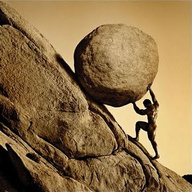
\includegraphics[width=0.4\textwidth]{determination}
      \end{center}
      \alert{\caption{determination}}
      \vspace{-20pt}
    \end{wrapfigure}
This has turned out to be the most important quality in startup founders. We thought when we started Y Combinator that the most important quality would be intelligence. That's the myth in the Valley. And certainly you don't want founders to be stupid. But as long as you're over a certain threshold of intelligence, what matters most is determination. You're going to hit a lot of obstacles. You can't be the sort of person who gets demoralized easily.}
\end{block}
\end{frame}
\section{Flexibility}
\begin{frame}{Flexibility}
        \begin{wrapfigure}{r}{0.5\textwidth}
        \vspace{-20pt}
      \begin{center}
        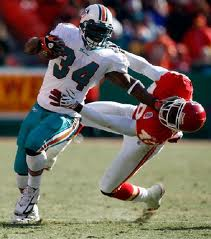
\includegraphics[width=0.4\textwidth]{runningback}
      \end{center}
      \alert{\caption{Running Back}}
      \vspace{-20pt}
    \end{wrapfigure}
  \begin{block}{You do not however want the sort of determination implied by phrases like "don't give up on your dreams." The world of startups is so unpredictable that you need to be able to modify your dreams on the fly. The best metaphor I've found for the combination of determination and flexibility you need is a running back. He's determined to get downfield, but at any given moment he may need to go sideways or even backwards to get there.}    
  \end{block}
\end{frame}
\section{Imagination}
\begin{frame}{Imagination}
        \begin{wrapfigure}{l}{0.5\textwidth}
      \vspace{-20pt}
      \begin{center}
        
\includegraphics[width=0.4\textwidth]{imagination}
      \end{center}
      \alert{\caption{Imagination}}
      \vspace{-20pt}
    \end{wrapfigure}
  \begin{block}{Intelligence does matter a lot of course. It seems like the type that matters most is imagination. It's not so important to be able to solve predefined problems quickly as to be able to come up with surprising new ideas. In the startup world, most good ideas seem bad initially. If they were obviously good, someone would already be doing them. So you need the kind of intelligence that produces ideas with just the right level of craziness.}
  \end{block}
\end{frame}
\section{Naughtiness}
\begin{frame}{Naughtiness}
      \begin{wrapfigure}{r}{0.5\textwidth}
      \vspace{-20pt}
      \begin{center}
        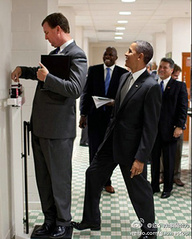
\includegraphics[width=0.38\textwidth]{naughtiness}
      \end{center}
      \alert{\caption{Naughtiness}}
      \vspace{-20pt}
    \end{wrapfigure}
  \begin{block}{Though the most successful founders are usually good people, they tend to have a piratical gleam in their eye. They're not Goody Two-Shoes type good. Morally, they care about getting the big questions right, but not about observing proprieties. That's why I'd use the word naughty rather than evil. They delight in breaking rules, but not rules that matter. This quality may be redundant though; It may be implied by imagination.}
  \end{block}
\end{frame}
\section{Friendship}
\begin{frame}{Friendship}
      \begin{wrapfigure}{r}{0.5\textwidth}
      \vspace{-20pt}
      \begin{center}
        
\includegraphics[width=0.48\textwidth]{friendship} 
      \end{center}
      \alert{\caption{Friendship}}
      \vspace{-20pt}
    \end{wrapfigure}
  \begin{block}{Empirically it seems to be hard to start a startup with just one founder. Most of the big successes have two or three. And the relationship between the founders has to be strong. They must genuinely like one another, and work well together. Startups do to the relationship between the founders what a dog does to a sock: if it can be pulled apart, it will be.}
  \end{block}
\end{frame}
\section{The End}
\begin{frame}{Q \& A}
\begin{center}
  \color{red}\LARGE{Thanks!}
\end{center}
\end{frame}
\end{CJK}
\end{document}
